\documentclass{article}%
\usepackage[T1]{fontenc}%
\usepackage[utf8]{inputenc}%
\usepackage{lmodern}%
\usepackage{textcomp}%
\usepackage{lastpage}%
\usepackage[head=40pt,margin=0.5in,bottom=0.6in]{geometry}%
\usepackage{graphicx}%
%
\title{\textbf{CIDH exigió al Estado respeto a la verdad y la justicia en el caso Albán}}%
\author{RAFAEL LEÓN | raleon@el{-}nacional.com}%
\date{06/12/2018}%
%
\begin{document}%
\normalsize%
\maketitle%
\textbf{URL: }%
http://www.el{-}nacional.com/noticias/politica/cidh{-}exigio{-}estado{-}respeto{-}verdad{-}justicia{-}caso{-}alban\_262285\newline%
%
\textbf{Periodico: }%
EN, %
ID: %
262285, %
Seccion: %
Política\newline%
%
\textbf{Palabras Claves: }%
NO\_TIENE\newline%
%
\textbf{Derecho: }%
18%
, Otros Derechos: %
1.1, 1.10, 1.2, 5%
, Sub Derechos: %
1.1.1.9, 1.10.1, 1.2.2%
\newline%
%
\textbf{EP: }%
NO\newline%
\newline%
%
\textbf{\textit{El comisionado Joel Hernández solicitó al gobierno que permita que el cuerpo del concejal metropolitano sea trasladado a Estados Unidos, para ser sepultado por su esposa e hijos}}%
\newline%
\newline%
%
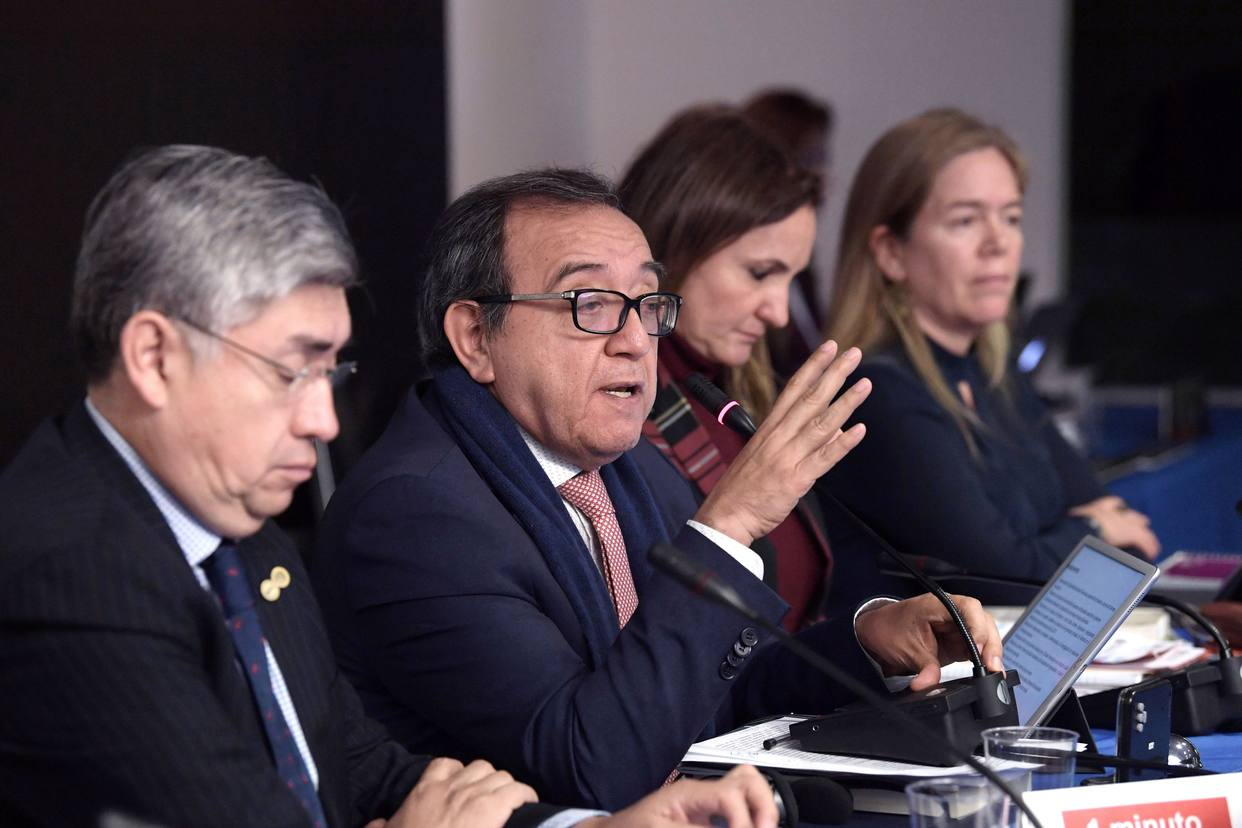
\includegraphics[width=300px]{232.jpg}%
\newline%
%
La Comisión Interamericana de Derechos Humanos exigió al Estado venezolano respetar el derecho al luto, la verdad y la justicia de la familia del concejal metropolitano Fernando Albán. También exhortó al gobierno a permitir una visita~in situ~para conocer la situación de los presos políticos y de los centros de reclusión.%
\newline%
%
La exigencia la hizo Joel Hernández, comisionado para las personas privadas de libertad, quien pidió investigar la verdad sobre la muerte del edil y que se entregue el cuerpo a su familia, que vive en Estados Unidos, para que sea sepultado.%
\newline%
%
Durante el 170 período de audiencias públicas de la CIDH, que se celebró ayer en Washington, Hernández tomó la petición de Meudy Osio, viuda del concejal, quien había solicitado al organismo interceder por el traslado de los restos, y la integración de una delegación de expertos independientes para investigar la muerte y las violaciones a los derechos humanos de las que habría sido víctima su esposo.%
\newline%
%
“Acudo ante ustedes para pedir justicia. Mis hijos y yo hemos perdido no solo a un padre y a un esposo, sino también a nuestra guía. A casi dos meses de su muerte no hay respuesta formal y creíble de lo que sucedió”, manifestó la viuda, en compañía de representantes de seis ONG, entre ellas, Sin Mordaza, Cepaz, Transparencia Venezuela, Codhez, Foro Penal y Defiende Venezuela.%
\newline%
%
Osio denunció que la detención arbitraria de Albán fue resultado de represalias por su participación en reuniones en la ONU, en septiembre. Señaló que la desaparición forzada, custodia y muerte en el Sebin está inmersa en irregularidades.%
\newline%
%
“El Estado venezolano tiene el deber de investigar, procesar y reparar la grave violación que constituye la muerte de Fernando Albán”, expresó Flavia Piovesan, comisionada para la comunidad LGTBI y las personas de la tercera edad.%
\newline%
%
El secretario ejecutivo del Consejo Nacional de Derechos Humanos de Venezuela, Larry Davoe, prometió trasladar las solicitudes de la CIDH al gobierno e insistió en que ya se han realizado “importantes” diligencias ~sobre “el lamentable suicidio”.%
\newline%
%
Persecución e impunidad. El grupo de ONG solicitó la audiencia para denunciar la situación de los derechos políticos y detenciones arbitrarias en Venezuela.%
\newline%
%
Los activistas denunciaron la eliminación de 90\% de los partidos opositores y expusieron los casos de persecución política a dirigentes y trabajadores.%
\newline%
%
Luis Armando Betancourt, representante del Foro Penal Venezolano, denunció que cada mes registran un promedio de 50 detenciones arbitrarias y que en los últimos 4 años ha habido más de 13.000 arrestos políticos.%
\newline%
%
“El gobierno de Venezuela viola los derechos humanos a través del sistema judicial: no cumple con el debido proceso, vulnera el derecho a la defensa, y atenta contra la integridad personal y psicológica de los detenidos”, manifestó.%
\newline%
%
Lavoe negó que en Venezuela se viole la libertad de expresión y de manifestación pacífica. “Todas las personas que se encuentran privadas de libertad cuentan con las garantías de sus derechos humanos”, expresó luego de presentar un video de Juan Requesens en la cárcel, con fotografías del diputado con sus familiares y recibiendo atención médica. En el audiovisual, el parlamentario afirma que no ha sido golpeado ni torturado y que se le brinda la atención médica requerida.%
\newline%
%
Rodrigo Diamanti, presidente de Sin Mordaza, dijo que la declaración del dirigente de Primero Justicia no tiene validez debido a que el video fue grabado bajo la custodia del Sebin.%
\newline%
%
“Me extraña que no mostraron el video del diputado con síntomas de tortura y lleno de excrementos. Este testimonio no tiene ningún tipo de validez porque ha sido grabado en un lugar donde han asesinado a personas y amenazan a los presos con atentar contra sus familiares”, expresó.%
\newline%
%
Oriana Granatti, esposa del parlamentario, reiteró la denuncia de violaciones contra del diputado. Indicó que estuvo 16 días con una infección bucal que le comprometió parte de la cara y no tuvo asistencia médica. “Juan es un diputado que tiene 120 días detrás de las rejas en El Helicoide. El gobierno solo quiere que los organismos internacionales crean que en Venezuela se respetan los derechos humanos, pero no es así. Juan es inocente y no debe estar allí”, expresó.%
\newline%
%
EL DATO%
\newline%
%
Tamara Sujú, abogada defensora de derechos humanos y directora del Instituto Casla, entregó a la Corte Penal Internacional el informe sobre torturas a ciudadanos durante 2018, ejecutadas por funcionarios de los cuerpos de seguridad del Estado. En el documento detallan 84 casos de 2017 y 106 de este año. Exponen los patrones de las violaciones cometidas por oficiales del Sebin y de la DGCIM, entre ellos, la asfixia mediante el uso de bolsas plásticas, la crucifixión de presos por 72 horas, descargas eléctricas, uso de gases lacrimógenos y casos de torturas psicológicas.%
\newline%
%
13 ONG exigen liberación inmediata del periodista alemán Billy Six%
\newline%
%
Un grupo de ONG suscribió un comunicado en el cual rechazan la detención arbitraria y el enjuiciamiento del periodista alemán Billy Six, en un tribunal militar, detenido el 17 de noviembre en Paraguaná cuando investigaba las actividades del narcotráfico, contrabando de combustible y material estratégico, trata de personas y el éxodo hacia el Caribe.%
\newline%
%
Las organizaciones exigieron al gobierno la liberación del comunicador extranjero, así como que se le garantice su integridad y restituyan los derechos violentados durante su reclusión. También denunciaron la arbitrariedad del procedimiento y la violación a las garantías de la libertad personal, el debido proceso y una legítima defensa.%
\newline%
%
“Rechazamos que se intente criminalizar la práctica periodística, en especial en un contexto crítico, en el cual la desinformación es promovida a través de las agresiones, ataques y amenazas a la labor reporteril y medios de comunicación nacionales y extranjeros”, expresa el documento firmado por las ONG Espacio Público, Expresión Libre y el Instituto de Prensa y Sociedad de Venezuela, entre otras.%
\newline%
%
Consideran que la aplicación de la justicia militar a civiles revela la lógica represiva del gobierno, viola el principio de separación de poderes y desconoce la legislación nacional, así como los tratados internacionales en materia de derechos humanos.%
\newline%
%
“Ante la ausencia de garantías de la libertad personal y el debido proceso” exhortan a los organismos internacionales y multilaterales de protección de derechos humanos a que activen los mecanismos necesarios ante la denuncia y realicen un llamado a la restitución de las garantías fundamentales de Six.%
\newline%
%
\end{document}